%% Source of figures/empirical-trend.pdf. Compile: pdflatex empirical-trend.tex
%% Generated 2026-10-28 from the SMOTE25 evaluation draft page (76 coded papers, 71 empirical).
%% Numbers are filled from the coded data; regenerate instead of editing them by hand.
\documentclass[border=4pt]{standalone}
\usepackage[scaled]{helvet}\renewcommand{\familydefault}{\sfdefault}
\usepackage{pgfplots}\pgfplotsset{compat=1.18}
\definecolor{sOne}{HTML}{2A78D6}\definecolor{sTwo}{HTML}{EB6834}\definecolor{sThree}{HTML}{1BAF7A}\definecolor{sFour}{HTML}{EDA100}
\definecolor{oZero}{HTML}{A3ABB4}\definecolor{oOne}{HTML}{5598E7}\definecolor{oTwo}{HTML}{1C5CAB}\definecolor{oThree}{HTML}{0D366B}\definecolor{inkTwo}{HTML}{465462}
\begin{document}
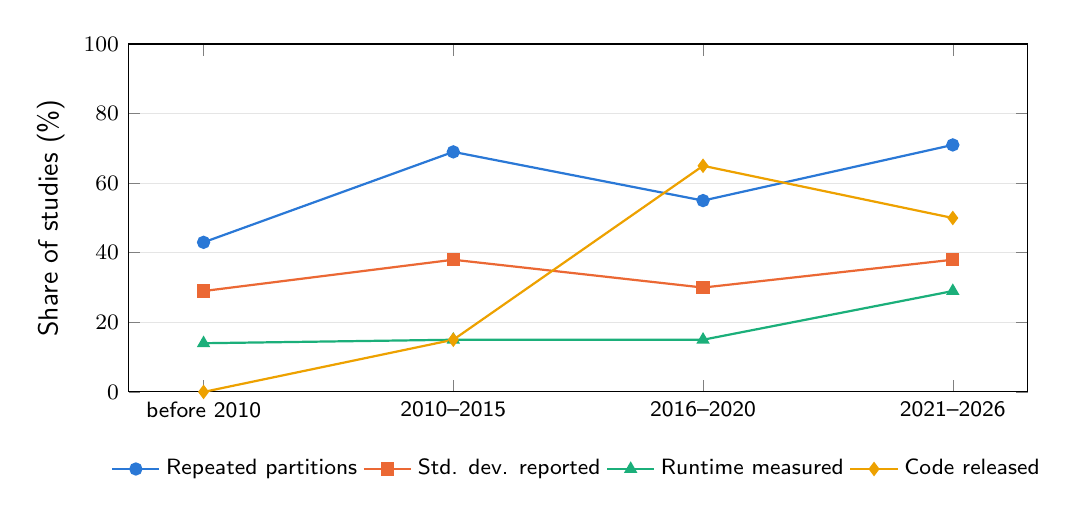
\begin{tikzpicture}
\begin{axis}[width=13cm,height=6cm,symbolic x coords={e1,e2,e3,e4},xtick=data,xticklabels={{before 2010},{2010--2015},{2016--2020},{2021--2026}},
  ymin=0,ymax=100,ylabel={Share of studies (\%)},tick label style={font=\footnotesize},legend cell align=left,legend style={font=\footnotesize,at={(0.5,-0.16)},anchor=north,legend columns=4,draw=none},ymajorgrids,grid style={gray!20}]
\addplot[thick,color=sOne,mark=*] coordinates {(e1,43) (e2,69) (e3,55) (e4,71)};
\addplot[thick,color=sTwo,mark=square*] coordinates {(e1,29) (e2,38) (e3,30) (e4,38)};
\addplot[thick,color=sThree,mark=triangle*] coordinates {(e1,14) (e2,15) (e3,15) (e4,29)};
\addplot[thick,color=sFour,mark=diamond*] coordinates {(e1,0) (e2,15) (e3,65) (e4,50)};
\legend{{Repeated partitions},{Std. dev. reported},{Runtime measured},{Code released}}
\end{axis}
\end{tikzpicture}
\end{document}
